% This is main.tex, a sample paper demonstrating the use of the
% LLNCS macro package for Springer Computer Science proceedings;
% Version 2.20 of 2017/10/04
% 
\documentclass[runningheads]{llncs}
%
% ---- Packages ----
%
\usepackage{graphicx} % enhanced support for graphics
\usepackage{url} % add macros for handling URLs in text
\usepackage[nohyperlinks,nolist]{acronym} % abbreviation utilities
\usepackage{listings}
% TODO: add more packages below if necessary
%
% ---- Acronyms ----
%
\begin{acronym}
\acro{rq}[RQ]{Research Question}
% TODO: define more acronyms here
\end{acronym}
%
% ---- Begin Document ----
%
\begin{document}
%
\title{Title of Seminar Paper}
%
%\titlerunning{Abbreviated paper title}
% If the paper title is too long for the running head, you can set
% an abbreviated paper title here
%
% ---- Author Information ----
%
\author{Jonas Schuhmacher, Jakob Rott}
\institute{Seminar: Software Quality (SS2022)\\
Technical University of Munich\\
\email{jonas.schuhmacher@tum.de, rott@cqse.eu}}
%
\maketitle % typeset the header of the contribution
%
% ---- Abstract ----
%
\begin{abstract}
The abstract should briefly summarize the contents of the paper in
15--250 words.

\keywords{First keyword  \and Second keyword \and Another keyword.}
\end{abstract}
%
% ---- Text Parts ----
%
\section{Introduction}
\label{sec:intro}

\subsection{Motivation}
\label{sec:intro:sub:motivation}

Please note that the first paragraph of a section or subsection is not indented.
The first paragraph that follows a table, figure, equation etc. does not need an indent, either.\footnote{Here is a sample footnote with a URL: \url{http://google.com}}

Subsequent paragraphs, however, are indented.

\subsubsection{Sample Heading (Third Level)} Only two levels of
headings should be numbered. Lower level headings remain unnumbered; they are formatted as run-in headings.

\paragraph{Sample Heading (Fourth Level)}
The contribution should contain no more than four levels of headings. 
Table~\ref{tab1} gives a summary of different text styles.

\begin{table}
\caption{Table captions should be placed above the
tables.}\label{tab1}
\centering
\begin{tabular}{|l|l|l|}
\hline
First col &  Second col & Third col\\
\hline
Normal & \textbf{Bold} & \textit{Italique}\\
\texttt{Typewriter} & \textsc{small caps} & \underline{underline}\\
\hline
\end{tabular}
\end{table}


\noindent Displayed equations are centered and set on a separate
line.
\begin{equation}
x + y = z
\end{equation}
Please try to avoid rasterized images for line-art diagrams and schemas. 
Whenever possible, use vector graphics instead (see Fig.~\ref{fig1}).

\begin{figure}
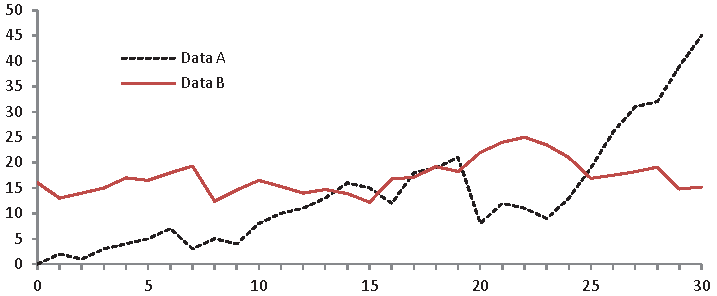
\includegraphics[width=\textwidth]{figures/fig1}
\caption{A figure caption is always placed below the illustration.
Please note that short captions are centered, while long ones are justified by the macro package automatically.} 
\label{fig1}
\end{figure}

\begin{theorem}
This is a sample theorem. 
The run-in heading is set in bold, while the following text appears in italics. 
Definitions, lemmas, propositions, and corollaries are styled the same way.
\end{theorem}
%
% the environments 'definition', 'lemma', 'proposition', 'corollary',
% 'remark', and 'example' are defined in the LLNCS documentclass as well.
%
\begin{proof}
Proofs, examples, and remarks have the initial word in italics, while the following text appears in normal font.
\end{proof}
For citations of references, we prefer the use of square brackets and consecutive numbers. 
Citations using labels or the author/year convention are also acceptable. 
The following bibliography provides a sample reference list with entries for journal articles~\cite{Stol2016}, a book~\cite{Myers2012}, conference proceedings~\cite{Harrold1988}, and a web site~\cite{Schaffer2018}.

\subsection{Abbreviations}
\label{sec:intro:sub:abbrev}

To use acronyms in the document, simple declare them in the main.tex file and use them later.
For example, you might want to define \acp{rq}, which will then be always abbreviated as \ac{rq} for singular or \acp{rq} for plural.

List are also really easy to create:

\begin{itemize}
  \item One entry in the list
  \item Another entry in the list
\end{itemize}

\begin{enumerate}
  \item The labels consists of sequential numbers.
  \item The numbers starts at 1 with every call to the enumerate environment.
\end{enumerate}

\subsection{Code Listings}
\label{sec:intro:sub:code}

Listings can either be created inside the text or imported:\footnote{See \url{https://www.overleaf.com/learn/latex/Code_listing} for a complete example.}
\begin{lstlisting}[language=C]
int main(int argc, char* argv[]) {
  return 0;
}
\end{lstlisting}
\section{Conclusion}
\label{sec:conclusion}

You can also reference other parts of the document, e.g., sections or subsections.
In Section~\ref{sec:intro} we briefly introduced something, whereas in Subsection~\ref{sec:intro:sub:motivation}, we motivated something else.

Make sure to capitalize chapters, sections or subsections when referencing them.
%
% ---- Appendix ----
%
\appendix
\section{Appendix}
\label{sec:appendix}

Anything additional goes here \dots
%
% ---- Bibliography ----
%
\bibliographystyle{splncs04}
\bibliography{library}
%
\end{document}
%
% ---- Begin Document ----
%
